\chapter{Appendix A}

\section{Additional Figures} \label{sec:additional_figures}

\begin{figure}[htpb]
    \centering
    \includesvg[width=0.75\linewidth]{Figures/C_p Distribution of Airfoil Wake at 0° AOA.svg}
    \caption[plot of the coefficient of pressure vs the angle of attack at zero degrees.]{Plot of \gls{C_P} distribution vs the Airfoils wake at an \acrshort{aoa} of \qty{0} {\degree}}
    \label{fig:C_p Distribution of Airfoil Wake at 0° AOA.svg}
\end{figure}

\begin{figure}[htpb]
    \centering
    \includesvg[width=0.75\linewidth]{Figures/C_p Distribution of Airfoil Wake at 4° AOA.svg}
    \caption[plot of the coefficient of pressure vs the angle of attack at four degrees.]{Plot of \gls{C_P} distribution vs the Airfoils wake at an \acrshort{aoa} of \qty{4} {\degree}}
    \label{fig:C_p Distribution of Airfoil Wake at 4° AOA.svg}
\end{figure}

\begin{figure}[htpb]
    \centering
    \includesvg[width=0.75\linewidth]{Figures/C_p Distribution of Airfoil Wake at 6° AOA.svg}
    \caption[plot of the coefficient of pressure vs the angle of attack at six degrees.]{Plot of \gls{C_P} distribution vs the Airfoils wake at an \acrshort{aoa} of \qty{6} {\degree}}
    \label{fig:C_p Distribution of Airfoil Wake at 6° AOA.svg}
\end{figure}

\begin{figure}[htpb]
    \centering
    \includesvg[width=0.75\linewidth]{Figures/C_p Distribution of Airfoil Wake at 8° AOA.svg}
    \caption[plot of the coefficient of pressure vs the angle of attack at eight degrees.]{Plot of \gls{C_P} distribution vs the Airfoils wake at an \acrshort{aoa} of \qty{8} {\degree}}
    \label{fig:C_p Distribution of Airfoil Wake at 8° AOA.svg}
\end{figure}

\begin{figure}[htpb]
    \centering
    \includesvg[width=0.75\linewidth]{Figures/C_p Distribution of Airfoil Wake at 10° AOA.svg}
    \caption[plot of the coefficient of pressure vs the angle of attack at 10 degrees.]{Plot of \gls{C_P} distribution vs the Airfoils wake at an \acrshort{aoa} of \qty{10} {\degree}}
    \label{fig:C_p Distribution of Airfoil Wake at 10° AOA.svg}
\end{figure}

\begin{figure}[htpb]
    \centering
    \includesvg[width=0.75\linewidth]{Figures/C_p Distribution of Airfoil Wake at 12° AOA.svg}
    \caption[plot of the coefficient of pressure vs the angle of attack at Twelve degrees.]{Plot of \gls{C_P} distribution vs the Airfoils wake at an \acrshort{aoa} of \qty{12} {\degree}}
    \label{fig:C_p Distribution of Airfoil Wake at 12° AOA.svg}
\end{figure}

\begin{figure}[htpb]
    \centering
    \includesvg[width=0.75\linewidth]{Figures/C_p Distribution of Airfoil Wake at 14° AOA.svg}
    \caption[plot of the coefficient of pressure vs the angle of attack at fourteen degrees.]{Plot of \gls{C_P} distribution vs the Airfoils wake at an \acrshort{aoa} of \qty{14} {\degree}}
    \label{fig:C_p Distribution of Airfoil Wake at 14° AOA.svg}
\end{figure}

\begin{figure}[htpb]
    \centering
    \includesvg[width=0.75\linewidth]{Figures/C_p Distribution of Airfoil Wake at 16° AOA.svg}
    \caption[plot of the coefficient of pressure vs the angle of attack at sixteen degrees.]{Plot of \gls{C_P} distribution vs the Airfoils wake at an \acrshort{aoa} of \qty{16} {\degree}}
    \label{fig:C_p Distribution of Airfoil Wake at 16° AOA.svg}
\end{figure}

\begin{figure}[htpb]
    \centering
    \includesvg[width=0.75\linewidth]{Figures/Magnitude of Airfoil C_d vs. AOA.svg}
    \caption[Plot of the magnitude of the coefficient of drag versus the angle of attack of an airfoil.]{Plot of the magnitude of the airfoil's \gls{C_d} vs. the airfoil's \acrshort{aoa}.}
    \label{fig:C_d_magnitude}
\end{figure}

\begin{figure}[htpb]
    \centering
    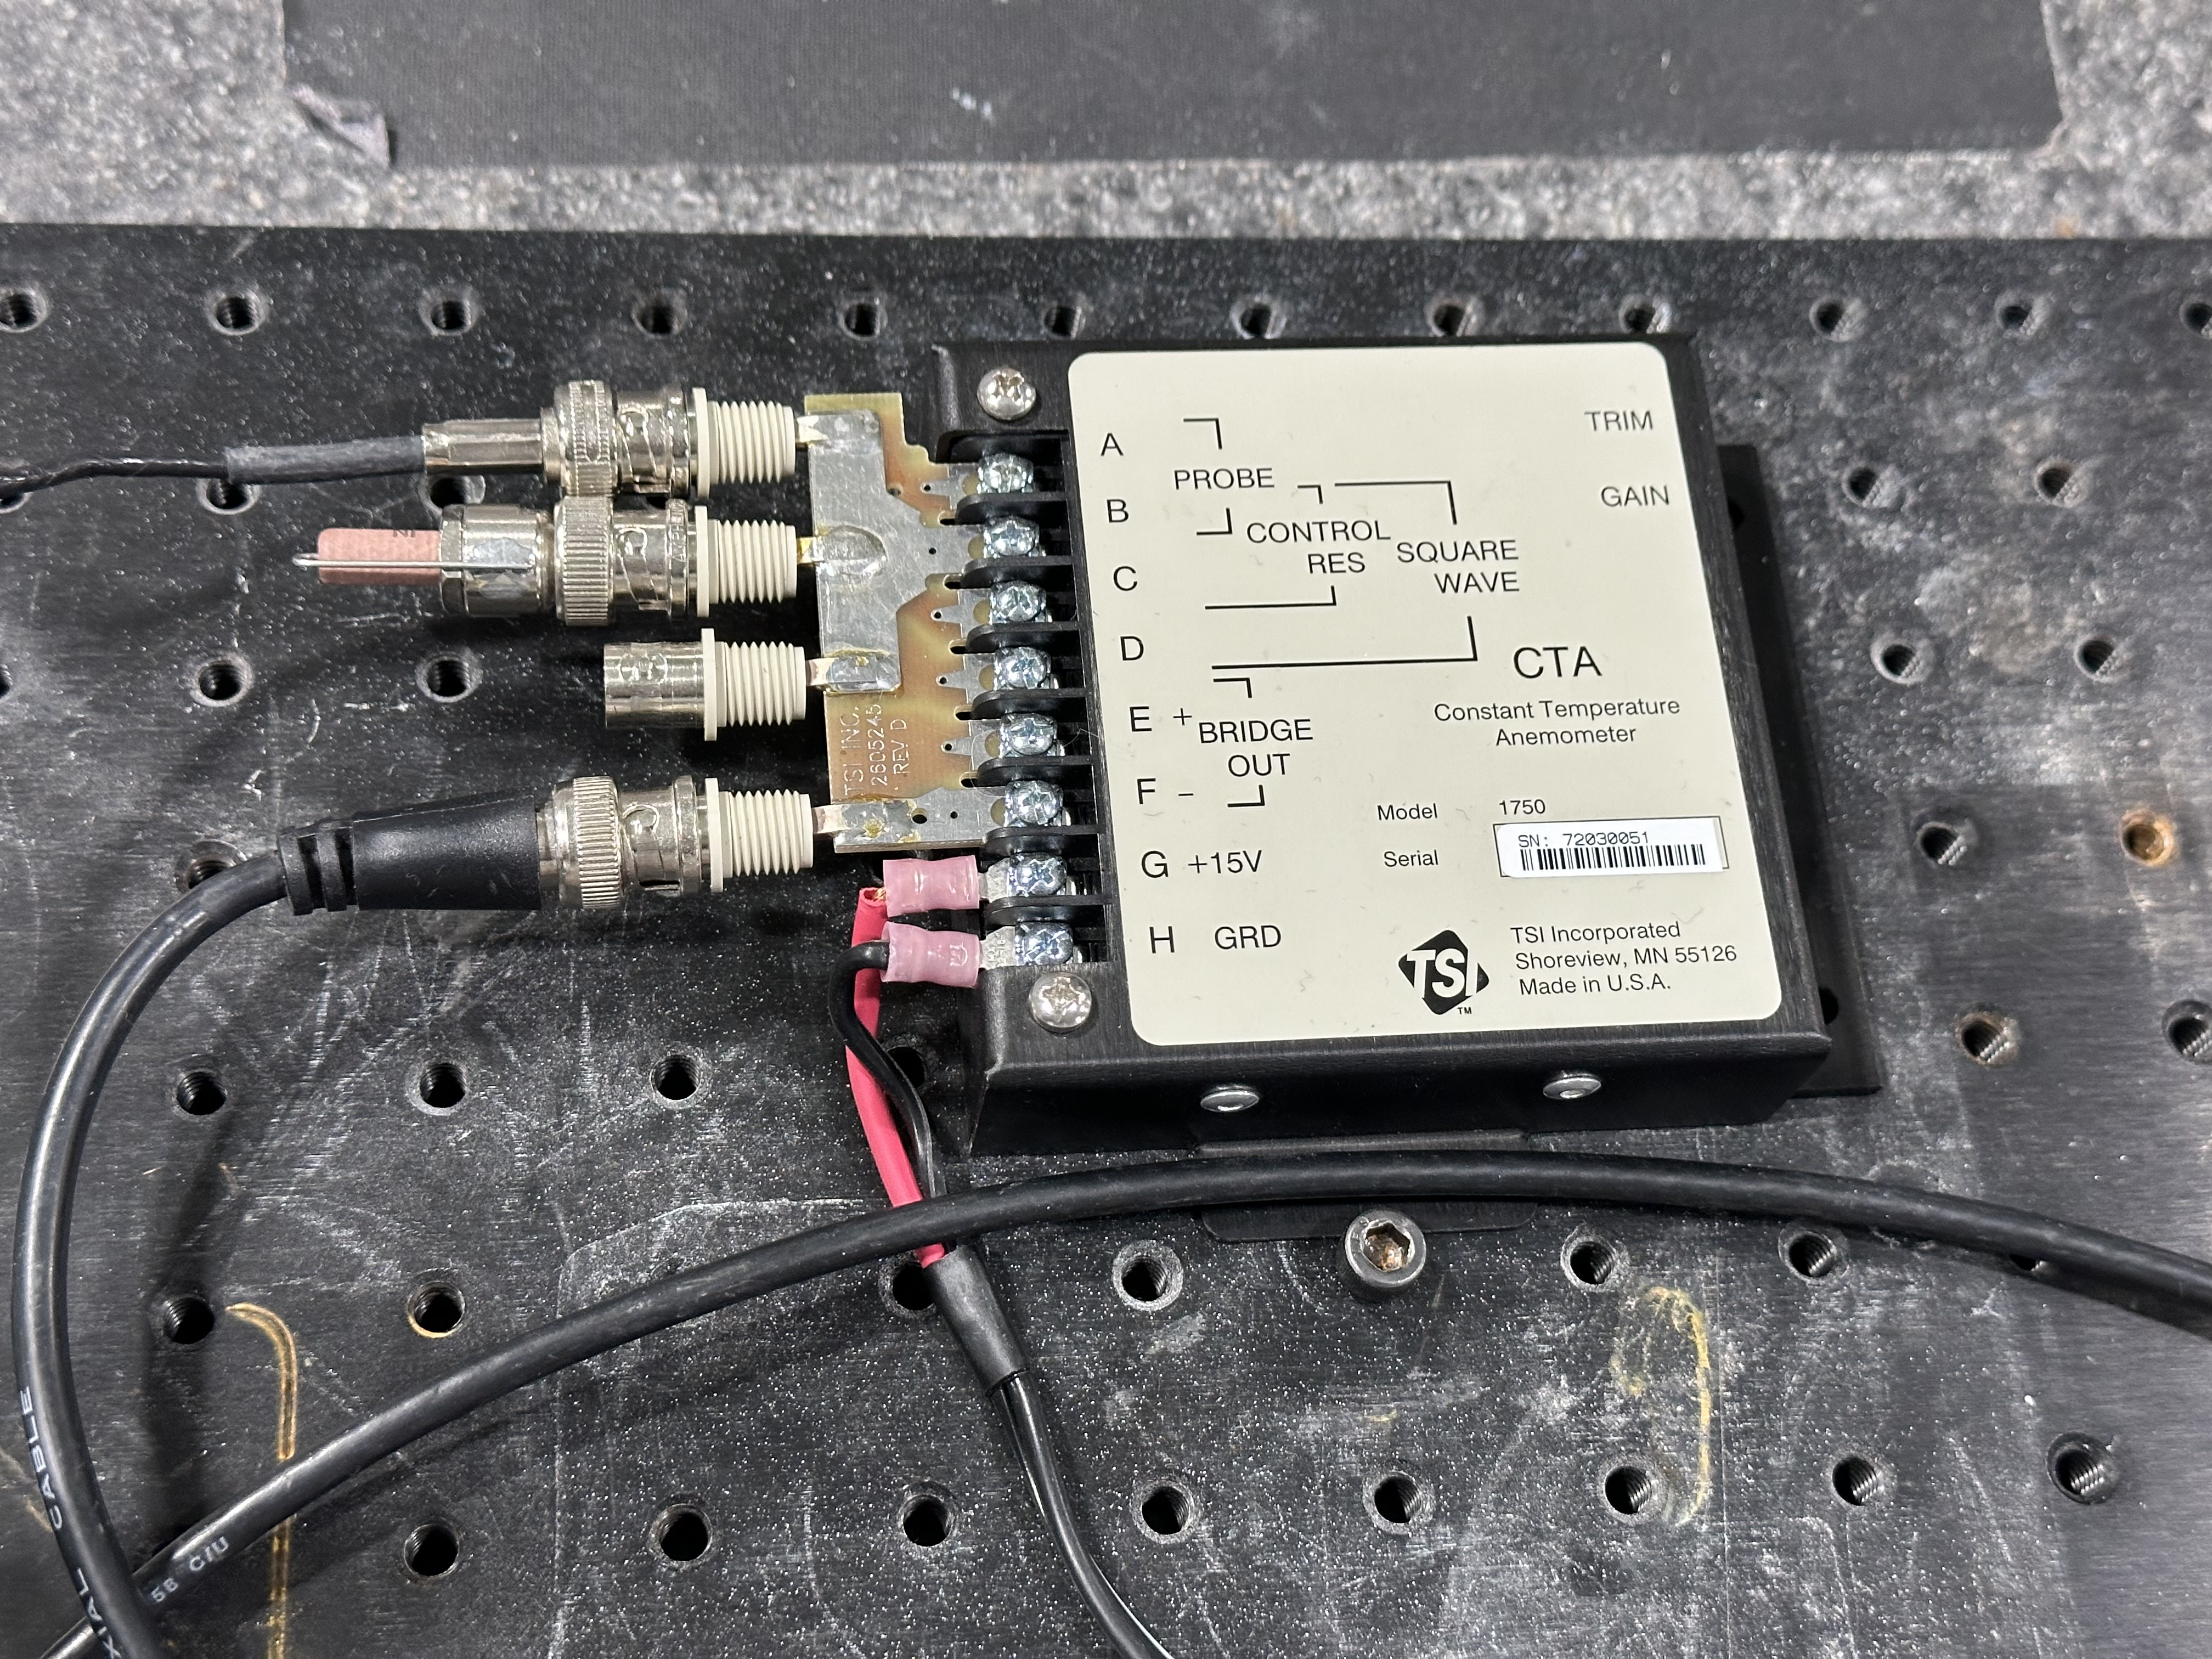
\includegraphics[width=0.75\linewidth]{Figures/IMG_3193.jpeg}
    \caption[Image of the Hot Wire data collection computer.]{Image of the Hot Wire data collection computer.}
    \label{fig: HotWireAndPitotComputer}
\end{figure}

\begin{figure}[htpb]
    \centering
    \includegraphics[width=0.75\linewidth]{Figures/IMG_3194.jpeg}
    \caption[Open loop wind tunnel speed controller and the Mensor manometer]{Open loop wind tunnel speed controller and the Mensor manometer}
    \label{fig: SpeedControl}
\end{figure}

\begin{figure}[htpb]
    \centering
    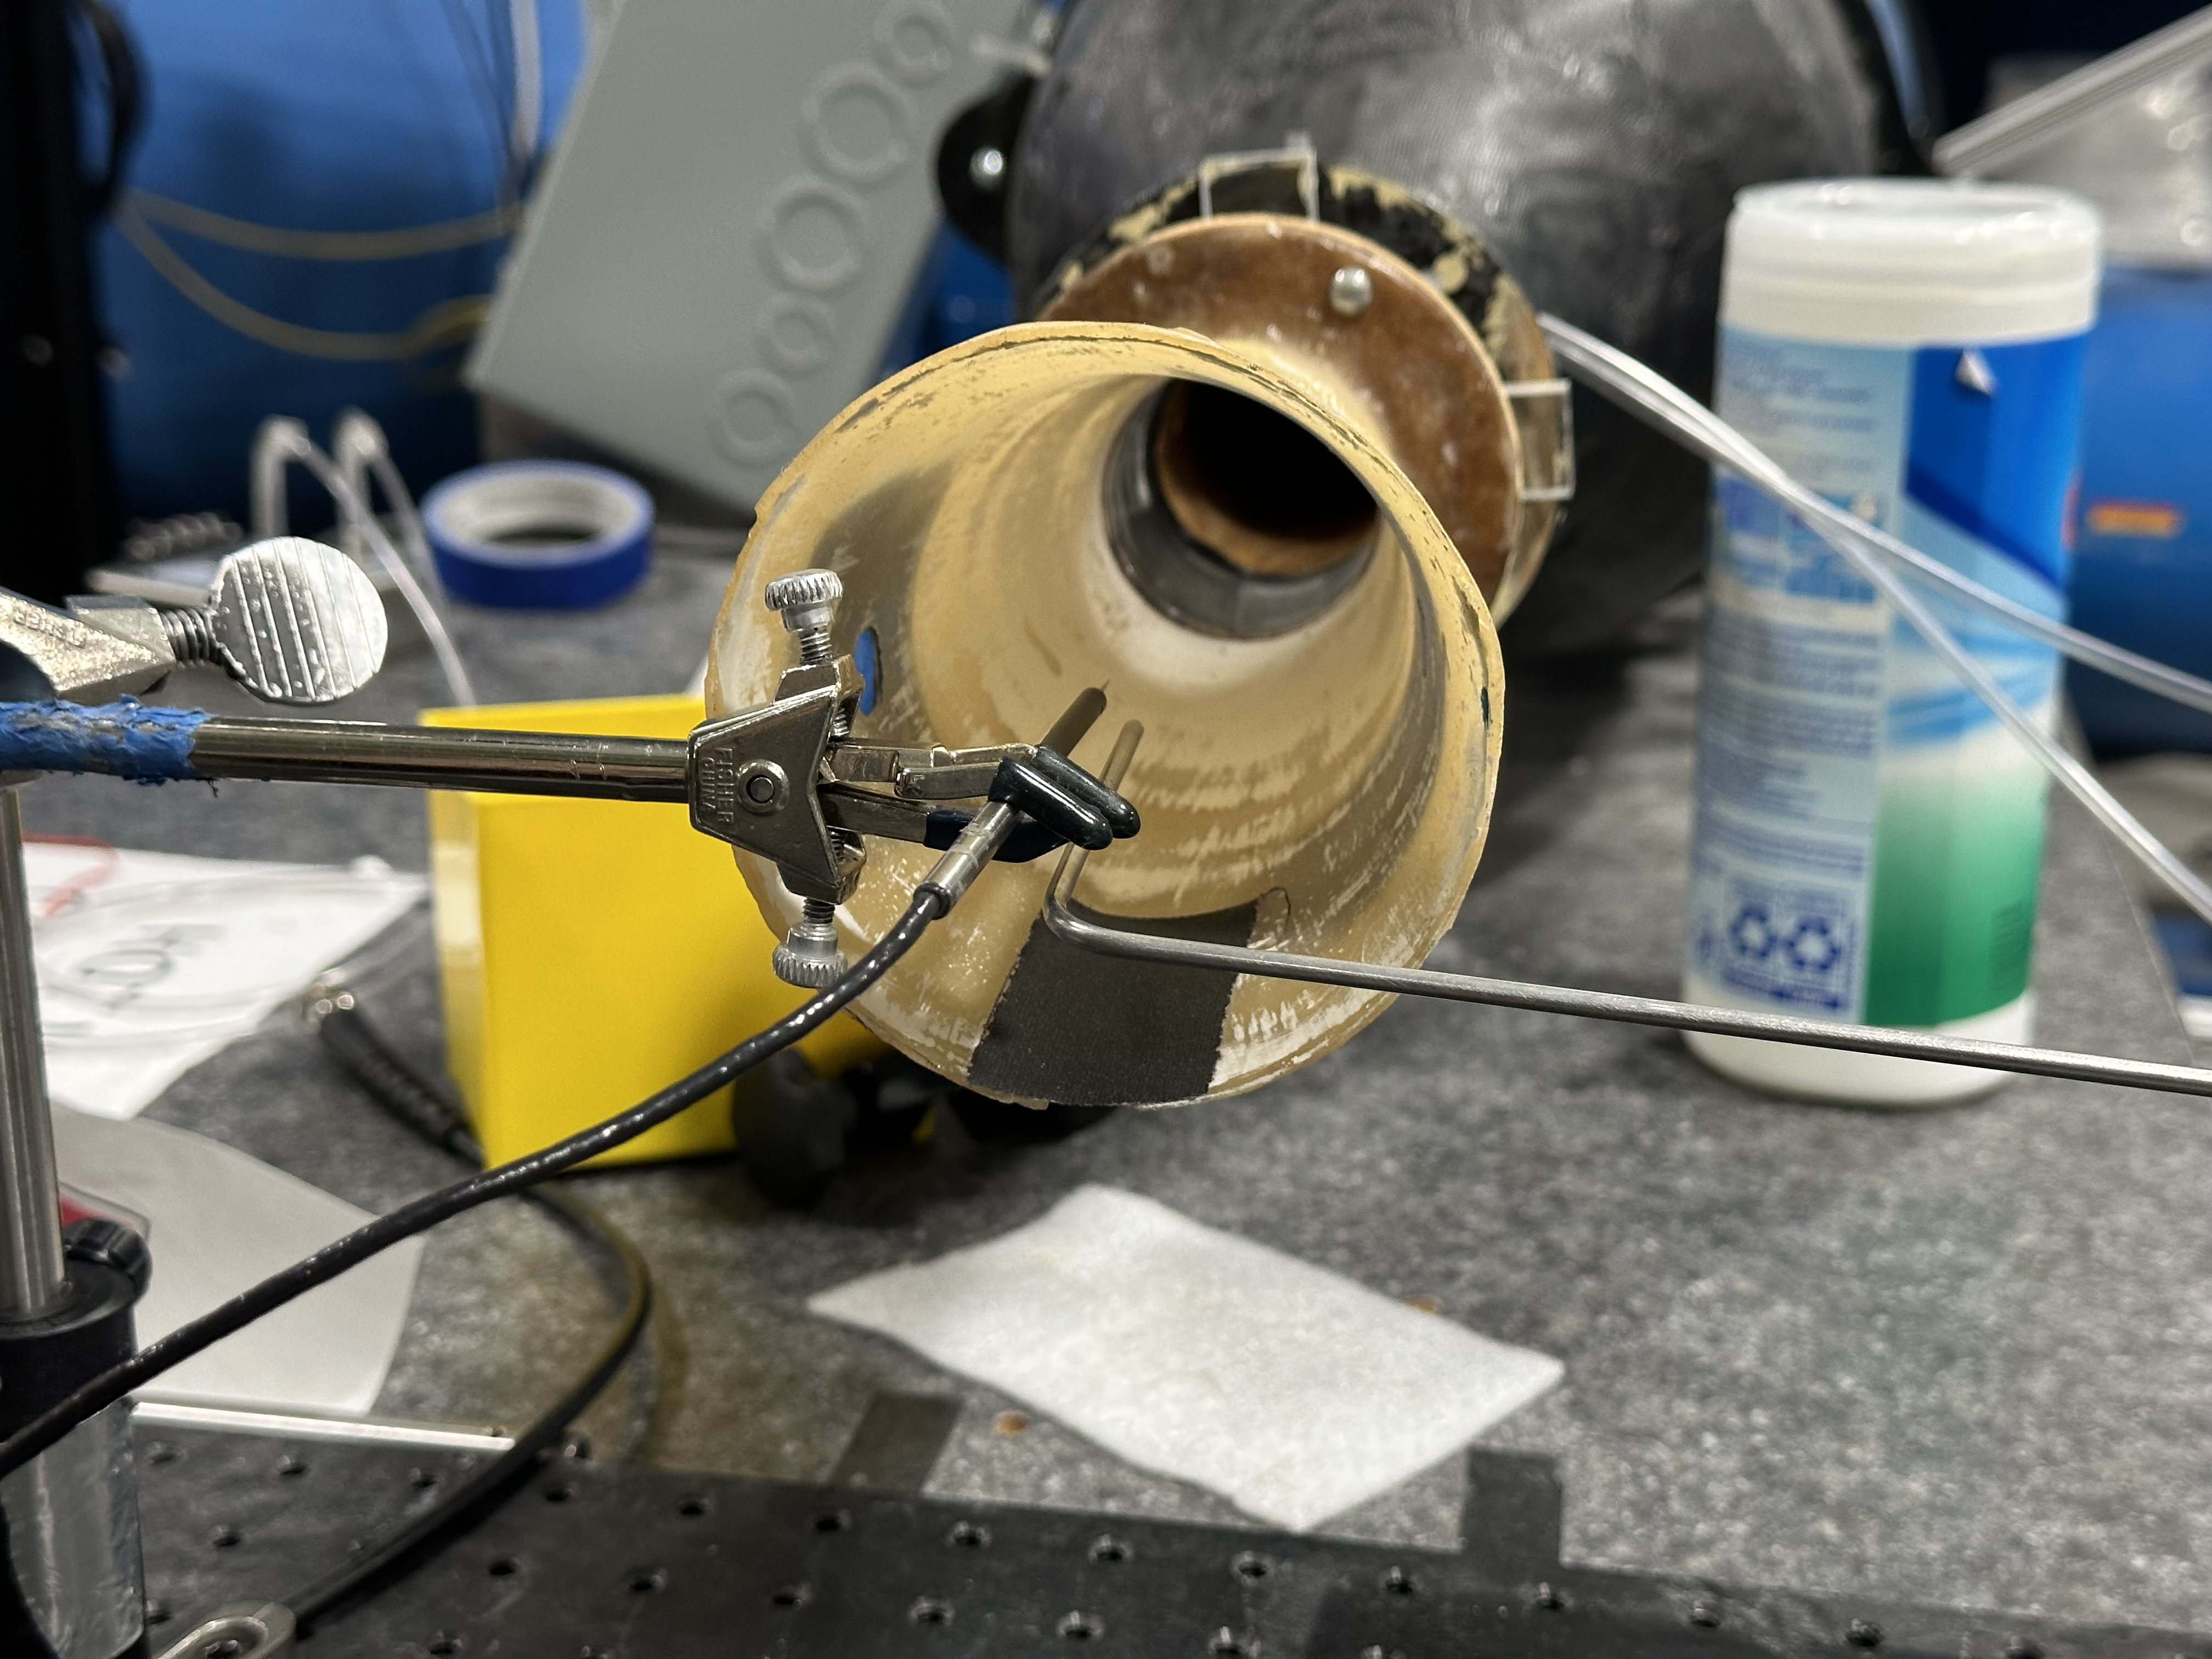
\includegraphics[width=0.75\linewidth]{Figures/IMG_3195.jpeg}
    \caption[Image of the Hot Wire Anemometer inside of open Circuit wind tunnel.]{Image of the Hot Wire Anemometer inside of open Circuit wind tunnel.}
    \label{fig: HotWireAndPitotFairPicture}
    \vspace*{5.5in}
\end{figure}


